% Springer Nature manuscript format (vendored under LPPL for a self-contained archive).
\RequirePackage{xr-hyper}
\documentclass[pdflatex,referee]{template/sn-jnl}
% A4 review layout: use the page instead of the class's small-format text block.
% Keep review line spacing; limit whitespace around figures and the title.
\geometry{reset,a4paper,left=22mm,right=24mm,top=20mm,bottom=22mm,
          bindingoffset=0mm,footskip=10mm}
\raggedbottom
\setlength{\floatsep}{10pt plus 2pt minus 2pt}
\setlength{\textfloatsep}{10pt plus 2pt minus 2pt}
\setlength{\intextsep}{10pt plus 2pt minus 2pt}
\renewcommand{\topfraction}{.95}
\renewcommand{\bottomfraction}{.90}
\renewcommand{\textfraction}{.05}
\renewcommand{\floatpagefraction}{.80}
\makeatletter
% Float-only pages start at the top instead of being vertically centred.
\setlength{\@fptop}{0pt}
\setlength{\@fpsep}{10pt plus 2pt minus 2pt}
\usepackage{etoolbox}
\patchcmd{\@maketitle}{\vskip21pt}{\vskip0pt}{}{}
% The class also inserts an empty opening box and an unused article-type row.
\patchcmd{\@maketitle}{\newpage\null}{\newpage}{}{\PackageError{synkit-layout}{Cannot remove title opening box}{Check the class title definition.}}
\patchcmd{\@maketitle}{{\hbox to \textwidth{{\Artcatfont\ArtType\hfill}\par}}}{}{}{\PackageError{synkit-layout}{Cannot remove unused article-type row}{Check the class title definition.}}
\patchcmd{\@maketitle}{\vskip20pt}{\vskip0pt}{}{\PackageError{synkit-layout}{Cannot remove title padding}{Check the class title definition.}}
\pretocmd{\Titlefont}{\def\baselinestretch{1}}{}{}
\patchcmd{\@maketitle}{\vskip36pt}{\vskip12pt}{}{}
\makeatother

% Capability marks for the software-scope table.  Defined here, in the shared
% preamble, because xr-hyper imports main.aux (and its caption) into the SI.
% Shape carries the meaning; the marks are distinguishable without colour.
\newcommand{\yes}{\ensuremath{\checkmark}}
\newcommand{\no}{\ensuremath{\times}}
\newcommand{\pmark}{\ensuremath{(\checkmark)}}
\newcommand{\rot}[1]{\rotatebox[origin=l]{90}{#1}}

% Shared TikZ figure styling, loaded after the document packages.
\AtEndPreamble{%
% Load in the document preamble. XeLaTeX/LuaLaTeX and an installed Arial
% family are required. Liberation Sans, metric-compatible with Arial, is the
% fallback where Arial is not installed.
\RequirePackage[no-math]{fontspec}
% Figures now use the text face, Latin Modern Roman, in a plain black-and-white
% print style. The family keeps its old name, \scArial, so the figure sources
% need no change. Only the visual abstract (a PDF from visual_abstract.py)
% keeps Arial and colour.
\newfontfamily\scArial{Latin Modern Roman}[NFSSFamily=scArial,Ligatures=TeX]
% Keep manuscript mathematics unchanged; select Arial letters and numerals
% only inside figures. TeX supplies specialist mathematical symbols.
\RequirePackage[subdued,italic]{mathastext}
\MTDeclareVersion{synarial}{TU}{scArial}{m}{n}
\SetMathAlphabet{\Mathsf}{synarial}{TU}{scArial}{m}{n}
\SetMathAlphabet{\Mathtt}{synarial}{TU}{scArial}{m}{n}

\usetikzlibrary{positioning,calc,fit,backgrounds,arrows.meta,shapes.geometric,
                shapes.misc,decorations.pathreplacing,patterns,math}

% --- canvas ---------------------------------------------------------------
% 372 pt text width minus the 1 pt standalone border on each side.
\newlength{\scW}\setlength{\scW}{13.0326cm}
\providecommand{\scWnum}{13.0326}
% \scCanvas{<height>} pins the picture to the full text width, y running down
% from 0, so every figure shares one coordinate convention.  It *sets* the
% bounding box rather than contributing to it, so the emitted page is exactly
% the text width and every figure is included at 1:1 -- otherwise a stray
% invisible extent (pgfplots reserves a little around an axis) rescales one
% figure relative to the others and the same \scSmall prints at two sizes.
% Anything drawn outside the canvas is therefore cropped: keep content inside,
% and check with
%     \providecommand{\scCanvas}[1]{\path[draw=red] (0,0) rectangle (\scWnum,-#1);}
\providecommand{\scCanvas}[1]{%
  \path[use as bounding box] (0,0) rectangle (\scWnum,-#1);}

% --- palette --------------------------------------------------------------
% Canonical companion-paper values (../../../../Style/style.tex).
% Black and white: the former hues map to ink and grays, so every figure
% prints the same in grayscale. Shape, fill, and dashing carry the meaning.
\definecolor{npgOrange}{gray}{0.35}
\definecolor{npgSky}{gray}{0.55}
\definecolor{npgGreen}{gray}{0}
\definecolor{npgYellow}{gray}{0.75}
\definecolor{npgBlue}{gray}{0}
\definecolor{npgVermillion}{gray}{0.45}
\definecolor{npgPurple}{gray}{0.4}
\definecolor{figInk}{gray}{0}
\definecolor{figMuted}{gray}{0.3}
\definecolor{figHair}{gray}{0.72}
\definecolor{figWash}{gray}{1}

\colorlet{scInk}{figInk}              % primary text
\colorlet{scInkM}{figMuted}           % secondary text
\colorlet{scPaper}{figWash}           % quiet cards and note strips
\colorlet{scSpF}{npgSky!12}           % species fill
\colorlet{scSpE}{npgBlue}             % species edge
\colorlet{scRxF}{npgOrange!12}        % reaction fill
\colorlet{scRxE}{npgOrange!88!black}  % reaction edge
\colorlet{scReac}{npgBlue!78!black}   % reactant edge
\colorlet{scProd}{npgGreen!82!black}  % product edge
\colorlet{scHiF}{npgOrange!13}        % highlight fill
\colorlet{scHiE}{npgOrange!82!black}  % highlight edge
% Stage / accent tints.  stDE remains available for the fifth plot series.
\colorlet{stAF}{npgGreen!9}\colorlet{stAE}{npgGreen}
\colorlet{stBF}{npgOrange!11}\colorlet{stBE}{npgOrange}
\colorlet{stCF}{npgBlue!9}\colorlet{stCE}{npgBlue}
\colorlet{stDF}{npgPurple!10}\colorlet{stDE}{npgPurple!85!black}
\colorlet{stEF}{npgVermillion!9}\colorlet{stEE}{npgVermillion}

% Semantic aliases.  Figures should speak in these, not in stAE/stBE/...
\colorlet{scAccent}{stAE}\colorlet{scAccentF}{stAF}   % structure / normal
\colorlet{scMark}{stBE}\colorlet{scMarkF}{stBF}       % highlight / certificate
\colorlet{scRef}{stCE}\colorlet{scRefF}{stCF}         % secondary series
\colorlet{scAlert}{stEE}\colorlet{scAlertF}{stEF}     % failure / violation
\colorlet{scRule}{figHair}                            % card and axis hairlines
\colorlet{scRuleL}{figHair!55}                        % grid, dividers

% --- text styles ----------------------------------------------------------
% Three sizes, fixed in points so they do not drift with the document class.
% Arial is shared by labels, headings, panel badges, and chemistry labels.
\providecommand{\scTitle}{\scArial\fontsize{8}{9.6}\selectfont\color{scInk}}
\providecommand{\scBody}{\scArial\fontsize{7}{8.4}\selectfont\color{scInk}}
\providecommand{\scSmall}{\scArial\fontsize{6.5}{7.8}\selectfont\color{scInk}}
\providecommand{\scSub}[1]{{\scSmall\itshape #1}}
\providecommand{\scPanel}[1]{{\scTitle(#1)}}
% Numerals that carry a result: ink, not colour, so the eye reads the value.
\providecommand{\scNum}{\scArial\fontsize{10}{11}\selectfont\bfseries\color{scInk}}

% --- shared TikZ styles ---------------------------------------------------
\tikzset{
  % text never hyphenates inside a figure
  every node/.append style={execute at begin node={%
      \hyphenpenalty=10000 \exhyphenpenalty=10000 \hbadness=10000 }},
  syn/.style={font=\scArial,color=scInk,
              execute at begin picture={\MTversion*{synarial}},
              >={Stealth[round,length=2.4mm,width=1.9mm]}},
  % containers ------------------------------------------------------------
  % One card chrome for the whole paper: white, 3 pt radius, one hairline.
  % Plain print style: panels, cards, notes and chips draw no frame.
  panel/.style={fill=none,draw=none},
  card/.style={fill=none,draw=none,inner sep=5pt,align=left,anchor=north west},
  note/.style={fill=none,draw=none,inner xsep=6pt,inner ysep=3.5pt,align=left,
               font=\scSmall},
  chip/.style={fill=none,draw=none,inner xsep=4pt,inner ysep=2pt,font=\scSmall},
  % Circular letter badge: the same accessible panel marker used in Style/*.
  hbullet/.style={circle,fill=scInk,text=white,draw=none,
                  font=\scArial\fontsize{6}{6}\selectfont\bfseries,
                  minimum size=4.2mm,inner sep=0pt},
  ctag/.style={font=\scTitle,anchor=north west,text=scInk},
  % CRN primitives --------------------------------------------------------
  species/.style={rounded rectangle,fill=scSpF,draw=scSpE,line width=0.45pt,
                  inner xsep=2.4pt,inner ysep=1.6pt,font=\scSmall,
                  text=scInk,minimum height=3.6mm},
  cofactor/.style={species,fill=scRefF,draw=scRef},
  catalyst/.style={species,fill=scHiF,draw=scHiE},
  rxn/.style={rectangle,fill=scRxF,draw=scRxE,line width=0.45pt,
              inner sep=1.2pt,font=\scSmall,text=scInk,
              minimum width=3.0mm,minimum height=3.0mm},
  place/.style={circle,fill=scSpF,draw=scSpE,line width=0.45pt,
                minimum size=4.0mm,inner sep=0pt},
  trans/.style={rectangle,fill=scRxE,draw=scRxE,minimum width=1.1mm,
                minimum height=3.6mm,inner sep=0pt},
  token/.style={circle,fill=scInk,minimum size=1.1mm,inner sep=0pt},
  % edges -----------------------------------------------------------------
  reac/.style={->,line width=0.5pt,draw=scReac,shorten >=0.8pt,shorten <=0.8pt},
  prod/.style={->,line width=0.5pt,draw=scProd,shorten >=0.8pt,shorten <=0.8pt},
  cat/.style={->,line width=0.5pt,draw=scHiE,shorten >=0.8pt,shorten <=0.8pt},
  flow/.style={-{Stealth[round,length=2.2mm,width=1.8mm]},line width=1.1pt,
               draw=scInkM!45},
  flab/.style={font=\scSmall,text=scInkM,inner sep=2pt},
  stoi/.style={font=\scSmall,text=scInkM,inner sep=0.8pt},
  % verdict marks: shape carries the meaning, colour only reinforces it
  vpass/.style={circle,fill=none,draw=none,text=black,
                font=\fontsize{6}{6}\selectfont\bfseries,
                minimum size=3.2mm,inner sep=0pt},
  vfail/.style={circle,fill=none,draw=none,text=black,
                font=\fontsize{6}{6}\selectfont\bfseries,
                minimum size=3.2mm,inner sep=0pt},
  callout/.style={font=\scSmall,text=scInkM,align=left},
}

% \scHead[<unused>]{<anchor coord>}{<letter>}{<title>}{<subtitle>}
% Plain "(a)" panel letter. Titles and subtitles are no longer printed: the
% caption names each panel. The arguments stay so the sources need no change.
\providecommand{\scHead}[5][scInk]{%
  \node[anchor=north west,inner sep=0pt,font=\scTitle] at #2
    {(\MakeLowercase{#3})};}

% --- shared pgfplots look (only if the figure loaded pgfplots) ------------
\ifdefined\pgfplotsset
  \pgfplotsset{compat=1.18}
  \pgfplotsset{
    synaxis/.style={
      scale only axis,
      tick align=outside, tick pos=left,
      axis line style={draw=scInkM!55,line width=0.4pt},
      % One grid, on the value axis only.  No minor grid: at these sizes it
      % turns the plot frame into a grey wash.
      ymajorgrids=true, xmajorgrids=false,
      major grid style={draw=scRuleL,line width=0.3pt},
      major tick length=1.6pt,
      label style={font=\scBody,color=scInk},
      tick label style={font=\scSmall,color=scInkM},
      legend style={font=\scSmall,draw=none,fill=none,inner sep=1pt,
                    row sep=0.4pt,legend columns=1},
      legend cell align=left,
      every axis plot/.append style={line width=0.7pt,mark size=1.2pt},
    },
  }
\fi

}


\usepackage[T1]{fontenc}
\usepackage{lmodern}
\usepackage{xspace}
\usepackage{graphicx}
\usepackage{xcolor}
\usepackage{listings}
\usepackage{booktabs}
\usepackage{microtype}
\usepackage{amsmath,amssymb}
\usepackage{mathrsfs}
\usepackage{subcaption}
\usepackage{float}
\usepackage{tabularx}
\usepackage{longtable}
\usepackage{array}
\usepackage{multirow}
\usepackage{pdflscape}
\usepackage{adjustbox}
\usepackage{enumitem}
\usepackage{siunitx}
\usepackage[version=4]{mhchem}
\usepackage{chemfig}
\usepackage{tikz}
\usepackage{pgfplots}

% Evidence figures are regenerated from JSON, and the glycolysis diagram uses TikZ.
% Shared figure styling is defined in paper_layout.tex.
\usepackage[numbers,square]{natbib}
\bibliographystyle{template/spbasic_u}

\newcommand{\synkit}{\texttt{SynKit}\xspace}
\newcommand{\synkitcrn}{\texttt{SynKit CRN}\xspace}
\hyphenation{SynKit Bio-in-for-mat-ics Reactome Wiki-Pathways}

% Help TeX avoid underfull lines in justified text
\emergencystretch=2em
\tolerance=2000
\hbadness=2000

% Listing settings
\lstset{
    basicstyle=\scriptsize\ttfamily\color{black},
    language=Python,
    keywordstyle=\color{blue},
    stringstyle=\color{olive},
    identifierstyle=\color{black},
    commentstyle=\color{gray},
    showstringspaces=false,
    frame=single,
    breaklines=true,
    breakatwhitespace=true,
    columns=fullflexible,
    keepspaces=true,
    upquote=true
}

\usepackage{hyperref}
\hypersetup{
  bookmarksdepth=2,
  colorlinks=true,
  linkcolor=blue,
  citecolor=blue,
  filecolor=blue,
  urlcolor=blue,
  anchorcolor=blue,
  pdfauthor={Thanh-An Pham and Tieu-Long Phan}
}

\externaldocument[supp:]{SI/si}

\begin{document}

\title[On The Conservation Laws and Pathway Realizability]{On The Conservation Laws and Pathway Realizability\hb of Biochemical Reaction Networks}

\author[1]{\fnm{Thanh-An} \sur{Pham}}\email{thanh-an.pham@uni-leipzig.de}
\author*[1,2]{\fnm{Tieu-Long} \sur{Phan}}\email{tieu@bioinf.uni-leipzig.de}

\affil[1]{\orgdiv{Bioinformatics Group, Department of Computer Science \& Interdisciplinary Center for Bioinformatics \& School for Embedded and Composite Artificial Intelligence (SECAI)}, \orgname{Leipzig University}, \orgaddress{\street{H{\"a}rtelstra{\ss}e 16--18}, \postcode{D-04107}, \city{Leipzig}, \country{Germany}}}
\affil[2]{\orgdiv{Department of Mathematics and Computer Science}, \orgname{University of Southern Denmark}, \orgaddress{\postcode{DK-5230}, \city{Odense M}, \country{Denmark}}}

% Generated numerical values shared with the supplement.
% BEGIN GENERATED: review-macros
% Generated from crn-review-experiments.json; do not edit.
\newcommand{\ReviewExhaustiveMilliseconds}{55.80}
\newcommand{\ReviewClosureMilliseconds}{1.47}
\newcommand{\ReviewRoundedFailures}{3}
\newcommand{\ReviewRatioSmall}{1.2}
\newcommand{\ReviewRatioLarge}{38.1}
\newcommand{\ReviewReversibleSiphonSeconds}{0.445}
\newcommand{\ReviewReversibleCanonicalSeconds}{0.495}
\newcommand{\ReviewReversibleMoietySeconds}{1.78}
\newcommand{\ReviewReversibleRankSeconds}{2.8}
\newcommand{\ReviewRandomSiphonSeconds}{0.161}
\newcommand{\ReviewRandomMoietySeconds}{0.0607}
\newcommand{\ReviewBioModelSiphonSeconds}{0.0323}
\newcommand{\ReviewBioModelMoietySeconds}{3.17}
\newcommand{\ReviewFormoseGenerationSeconds}{0.0144}
% END GENERATED: review-macros

% BEGIN GENERATED: glycolysis-macros
% Generated by glycolysis_analysis.py; do not edit by hand.
\def\GlySpecies{14}
\def\GlyReactions{15}
\def\GlyComplexes{16}
\def\GlyLinkage{4}
\def\GlyRank{11}
\def\GlyDeficiency{1}
\def\GlyMoieties{3}
\def\GlyBackboneSupport{11}
\def\GlySiphons{3}
\def\GlyUncovered{2}
\def\GlyCertificateLength{15}
\def\GlyExplored{30}
\def\GlyDepth{15}
\def\GlyUpperFirings{5}
\def\GlyLowerFirings{10}
\def\GlySplitStep{4}
\def\GlyTrajectory{0/1/2,1/1/2,2/1/2,3/1/2,4/2/2,5/2/2,6/2/2,7/2/2,8/2/2,9/2/2,10/2/2,11/2/2,12/2/2,13/2/2,14/2/2,15/2/2}
% END GENERATED: glycolysis-macros

% BEGIN GENERATED: hydrogen-macros
% Generated from crn-hydrogen.json; do not edit.
\newcommand{\HydrogenDepth}{6}
\newcommand{\HydrogenSpecies}{10\,572}
\newcommand{\HydrogenReactions}{11\,239}
\newcommand{\HydrogenExplicitSeconds}{9.0}
\newcommand{\HydrogenLewisSeconds}{5.9}
\newcommand{\HydrogenLewisReactions}{23}
\newcommand{\HydrogenInsertionExplicit}{12}
% END GENERATED: hydrogen-macros
\abstract{
\textbf{Background:} Conserved metabolite pools and substrate availability constrain biochemical pathways before kinetic parameters are known. Analyzing these constraints across curated and rule-generated networks requires both reaction stoichiometry and the amounts of substrates consumed at each step. Species that appear on both sides of a reaction cancel from the net stoichiometry, although the reaction still needs them to fire.

\textbf{Results:} We present the chemical reaction network (CRN) submodule of \synkit, an open-source Python toolkit, for constructing biochemical reaction networks and analyzing their conserved pools, chemical reaction network theory (CRNT) properties, and realizable reaction sequences. \texttt{KEGG} pathways, supported \texttt{SBML} models, and rule-generated reactions use the same reaction records. Twelve reference networks pass the validation checks and agree with \texttt{CRNT4SBML} on eight shared structural quantities. Ten reaction-bearing \texttt{BioModels} entries pass structural \texttt{SBML} round trips, including a model with 504 species and 827 directed reactions. Four \texttt{KEGG} modules illustrate conserved pools and the effects of model boundaries. In glycolysis, removing shared polyphosphate from a reaction changes deficiency and substrate requirements while preserving the net stoichiometric matrix. A 15-step glucose-to-pyruvate firing sequence is realizable after currency metabolites are removed but is blocked from glucose alone when they are retained. In a generated formose network, conservation coefficients match carbon counts for all 37 species, but equal carbon inventories differ in their ability to supply the selected tetrose and hexose routes. Native rule expansion that keeps hydrogens as per-atom counts reproduces this network exactly and conserves atoms and charge in every reaction of three hydrogen-transfer controls, where re-deriving hydrogens from default valences does not. C++ implementations complete all reported structural enumerations, including all 60 configurations of the scaling study.

\textbf{Conclusions:} \synkit brings conservation analysis and reaction-by-reaction realizability checks to the same biochemical model. Its results help distinguish conserved quantities, unmet substrate requirements, and the assumptions needed for CRNT conclusions. Source code, recorded results, and reproducible analyses accompany the manuscript.
}
\keywords{Chemical reaction networks, chemical reaction network theory, Petri nets, conserved moieties, stoichiometry, pathway realizability, \texttt{SBML}}
\maketitle

\section{Background}
\label{sec:intro}

Curated databases such as \texttt{KEGG}~\cite{kanehisa2025kegg}, \texttt{Reactome}~\cite{ragueneau2026reactome}, and \texttt{WikiPathways}~\cite{agrawal2024wikipathways} provide biochemical reaction records for reuse, while graph-transformation methods enumerate candidate reactions from molecular seeds and transformation rules~\cite{andersen2016mod}. Before assigning kinetic parameters, researchers need to determine which quantities a network conserves, which structural theorems apply, and whether a proposed route can fire from the available substrates. Answering these questions on the same reaction system is useful for checking metabolic modules and screening generated reaction spaces.

These analyses require different information. A species graph represents connectivity but can lose the joint requirement of multiple substrates~\cite{franzese2019hypergraph}. The net stoichiometric matrix records changes in species amounts but cancels species present on both sides. Over the same species set, $A+C\to B+C$ and $A\to B$ have identical net columns, yet only the first needs $C$ to fire, and the two have different complexes. Similarly, a balanced reaction combination or a qualitatively reachable product does not establish that the reactions can fire in an admissible order from a finite inventory~\cite{andersen2023realisability}. Conversion choices can therefore preserve one analysis while changing another.

Existing packages address subsets of these tasks. \texttt{COBRApy}~\cite{ebrahim2013cobrapy} supports metabolic reconstruction and constraint-based flux analysis, including flux balance analysis~\cite{orth2010fba} and elementary flux modes~\cite{schuster1994efm}. \texttt{CRNT4SBML}~\cite{reyes2020crnt4sbml} provides deficiency analysis and bistability detection. \texttt{M\O D}~\cite{andersen2016mod} combines graph rewriting with reaction-space exploration, and \texttt{Tellurium}~\cite{choi2018tellurium} and \texttt{libRoadRunner}~\cite{welsh2023libroadrunner} support kinetic simulation. Petri-net representations of metabolic networks are widely used in structural analysis~\cite{zevedei2003topological,murata1989petri} and provide pathway realizability certificates~\cite{andersen2023realisability}. \texttt{SBML}~\cite{hucka2003sbml} and \texttt{COMBINE}~\cite{bergmann2014combine} standardize model exchange, while converters such as \texttt{KEGGtranslator}~\cite{wrzodek2011keggtranslator} export curated pathways into \texttt{SBML}. However, file conversion alone does not guarantee that the structural assumptions required for each analysis are preserved.

Conserved pools and substrate sufficiency need to be examined on the same imported or generated reaction list. A glycolytic route may appear connected from glucose to pyruvate when ATP and redox cofactors are ignored, yet fail to fire when those cofactors are retained as required reactants with limited initial supplies. In a generated carbohydrate network, every reaction may conserve carbon, yet a proposed pathway may remain unrealizable because its reactions require more glycolaldehyde molecules than the initial inventory contains. In both cases, network structure and conservation laws alone do not establish that the sequence can run from the specified finite inventory.

We developed the chemical reaction network (CRN) submodule of \synkit~\cite{phan2025synkit} to run these checks on a shared reaction record. It connects \texttt{KEGG} ingestion, structural \texttt{SBML} exchange, and rule-based construction to exact conservation and deficiency calculations, Petri-net siphon analysis, and replayable firing certificates, while reporting the hypotheses required by each conclusion. We validate the submodule on twelve reference networks, compare eight shared structural quantities against \texttt{CRNT4SBML}, test structural round trips on ten \texttt{BioModels} entries spanning two orders of magnitude in size, and measure the cost of exact enumeration. Controlled experiments in glycolysis and in a rule-generated formose network then isolate how participant cancellation, cofactor boundaries, and precursor mixtures alter deficiency and pathway realizability even when net stoichiometry or total carbon is unchanged.

\section{Implementation}
\label{sec:description}

\subsection{Reaction-network construction and representation}
\label{sec:acquisition}
\label{sec:representation}

Within the CRN submodule, \texttt{SynCRN} stores species, reactions, rules, and source annotations as reaction records. It derives a \texttt{NetworkX}-compatible bipartite digraph, stoichiometric matrices, a Petri net, and reaction equations on demand (Figure~\ref{fig:synkit_architecture}). The graph partitions species $X$ and reactions $\mathscr{R}$, where species-to-reaction and reaction-to-species edges encode consumption and production. Reading each reaction and its incident edges as a directed hyperedge preserves multi-substrate dependencies.

For reaction $r$, the reactant and product multisets have coefficients $s^-_{xr}$ and $s^+_{xr}$. The integer-stoichiometry analyses in this paper use
\begin{equation}
\mathbf S^-=(s^-_{xr}),\quad \mathbf S^+=(s^+_{xr}),\quad
\mathbf S=\mathbf S^+-\mathbf S^-.
\end{equation}
Shared participants remain in both incidence matrices. Cancelling equal coefficients preserves $\mathbf S$ but can change reaction enabling and the complex graph. In Petri-net terms, a species on both sides of a reaction forms a self-loop, and the incidence matrix of a net with self-loops (an impure net) does not determine when its transitions are enabled~\cite{murata1989petri}. Construction does not establish elemental balance automatically, so chemical interpretation requires suitable input equations and annotations, and the conditions under which a reaction network is chemically realizable are themselves a subject of study~\cite{muller2022chemical}.

The \texttt{Query} adapter parses \texttt{KEGG} equations, \texttt{Construct} expands seed molecules using \texttt{SMARTS} or double-pushout graph rules, and \texttt{IO} imports supported \texttt{SBML} Core reaction structure. Reversible equations can become two directed reactions. Omitting currency metabolites, such as ATP, NADH, water, or protons, or excluding boundary species changes the analyzed system. These choices are specified when constructing the network. The \texttt{Symmetry} module combines Weisfeiler--Lehman color refinement~\cite{shervashidze2011weisfeiler} with exact graph methods for canonicalization, isomorphism, and automorphism analysis~\cite{junttila2007bliss,mckay2014practical}. Automorphisms reflect graph structure unless species labels are fixed during matching.

\begin{figure}[!htbp]
\centering
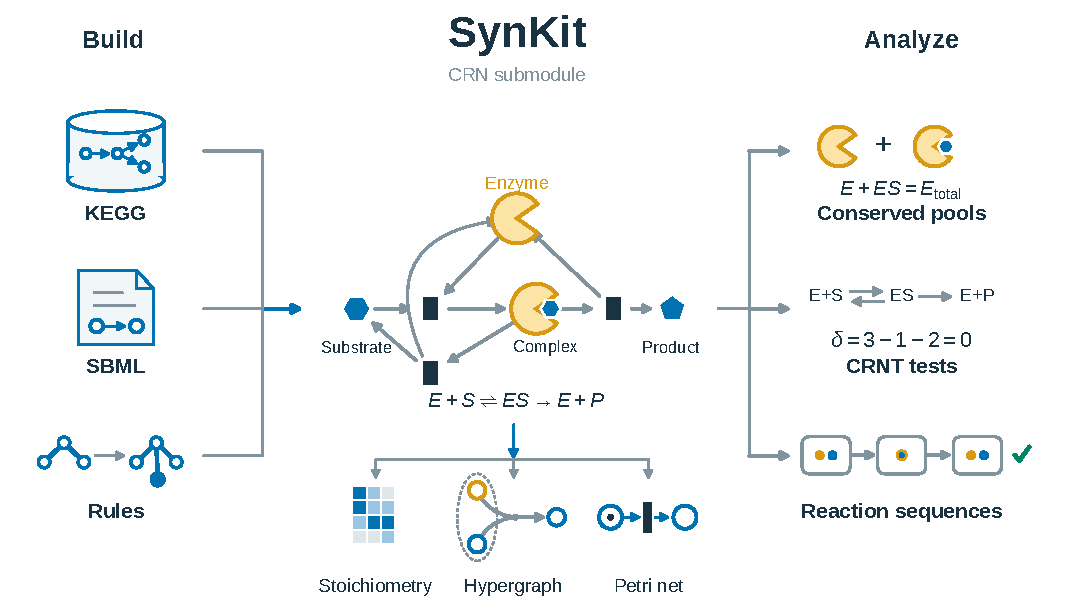
\includegraphics[width=\linewidth]{Figure/visual_abstract.pdf}
\caption{Reaction representation and structural analysis workflows in \texttt{SynKit CRN}. Curated pathways (\texttt{KEGG}), models (\texttt{SBML}), and reaction rules map to a shared bipartite representation. An illustrative enzyme scheme ($E+S\rightleftharpoons ES\to E+P$, with conserved pool $E+ES$) yields stoichiometric, hypergraph, and Petri-net views for exact conservation analysis, CRNT theorem checks, and discrete pathway realizability. Circles denote species and dark bars reactions. The hypergraph view shows one directed hyperedge whose tail set $\{E,S\}$ is consumed jointly. The deficiency and the firing sequence ($E+S\to ES\to E+P$) shown on the right are those of the example. Molecular and diagram icons are schematic. Blue marks species, orange the enzyme, and green a verified result. The other figures are printed in black and white.}
\label{fig:synkit_architecture}
\end{figure}

\subsection{Exact stoichiometric analysis and conserved pools}
\label{sec:analysis}

The stoichiometric matrix $\mathbf S$ records the net change in every species for each reaction. For concentrations $c$ and reaction rates $v(c)$, the dynamics are written as $\dot c=\mathbf S v(c)$. A vector $y$ satisfying $y^T\mathbf S=0$ defines a conserved linear quantity $y^Tc$, because the reactions can redistribute the participating species without changing this weighted total. \synkitcrn computes a rational basis for the left nullspace of $\mathbf S$ and converts its vectors to primitive integer representatives. These vectors describe all rational conservation relations, but they need not be non-negative or identify the smallest conserved pools.

Minimal P-semiflows are computed separately by exact Farkas elimination~\cite{colom1991convex}. They are non-zero, non-negative integer vectors in the left kernel of $\mathbf S$ with inclusion-minimal supports, normalized by their greatest common divisor. Their supports identify minimal conserved pools of the represented network~\cite{famili2003leftnullspace}. A P-semiflow guarantees mathematical conservation, whereas assigning its support to a chemical moiety requires species annotations and biochemical interpretation.

T-semiflows satisfy $\mathbf Sx=0$ with $x\ge0$ and describe balanced combinations of reactions whose total net species change is zero. They are reaction-space relations, not conserved species pools. A T-semiflow fixes neither a firing order nor an initial marking, and it does not imply thermodynamic feasibility. All-positive left and right kernel vectors define conservativity and consistency, respectively. For positive-kernel feasibility, a numerical linear program proposes a witness, which is accepted only after exact integer or rational verification. Verified positive answers include an all-positive kernel vector, negative answers include a rational separating vector, and unverified solver outcomes remain undecided. Numerical kernel and Jacobian-pattern checks are also available. These describe approximations or possible matrix entries. In particular, a floating-point nullspace basis can represent a subspace accurately without identifying integer minimal supports, so naively rounding such a basis is not a substitute for exact conservation-law computation.

\subsection{Network deficiency and steady-state theorem applicability}
\label{sec:crnt}

Complexes are distinct reactant or product multisets. With $n$ complexes, $\ell$ connected components of the complex graph (linkage classes), and stoichiometric rank $s$, deficiency is $\delta=n-\ell-s$.
A network is weakly reversible when every linkage class is strongly connected. \synkitcrn calculates ranks exactly over $\mathbb Q$ and reports the deficiency of the network and of each linkage class, weak reversibility, and the terminal strong linkage classes.

For positive mass-action rate constants, a weakly reversible deficiency-zero network has exactly one positive steady state in each positive stoichiometric compatibility class $(c_0+\operatorname{im}\mathbf S)\cap\mathbb R^{X}_{>0}$, and it is locally asymptotically stable relative to that class~\cite{horn1972general,feinberg1987deficiency}. A deficiency-zero network that is not weakly reversible has no positive steady state. The Deficiency One Theorem gives at most one positive steady state per positive stoichiometric compatibility class when each linkage-class deficiency is at most one, their sum equals $\delta$, and each linkage class has one terminal strong linkage class, while weak reversibility additionally ensures existence~\cite{feinberg1995existence}. Failure of these hypotheses leaves the corresponding theorem undecided. Introductions to this body of theory for biologists are available~\cite{gunawardena2003crnt}. Criteria that reach beyond deficiency, including injectivity~\cite{craciun2005injectivity}, concordance~\cite{shinar2012concordant}, and graph-theoretic multistationarity tests~\cite{mincheva2007graph1}, are not implemented here, and a network left undecided by the deficiency theorems is not thereby shown to be multistationary. The Edelstein example in Supplementary Figure~\ref{supp:fig:deficiency} illustrates this distinction.

\subsection{Petri-net analysis and discrete pathway realizability}
\label{sec:petrinet}
\label{sec:pathway}

A siphon is a non-empty species set for which every reaction producing a member also consumes a member. Once empty, it cannot refill under Petri-net firing semantics. A trap has the dual property that every reaction consuming a member also produces a member, so a marked trap cannot become empty~\cite{murata1989petri}. \synkitcrn enumerates minimal siphons using implication propagation and closure minimization, within the branch-and-bound approach to structural enumeration~\cite{cordone2005enumeration}. Producing a selected species forces selection of a reactant. Selected and excluded species are propagated before branching. Each reported minimal set excludes its supersets from further search, and a maximal-closure deletion test verifies minimality. Traps use the dual incidence. This prunes many subsets but does not remove worst-case combinatorial growth.

The package checks whether every minimal siphon contains the support of a P-semiflow, and we call such a siphon covered. Under the boundedness and kinetic assumptions of the corresponding persistence result, this provides a sufficient persistence certificate for positive initial conditions~\cite{angeli2007persistence}. An uncovered siphon means the test is insufficient, and does not prove extinction or identify a unique nutrient supplementation strategy. The returned details expose these uncovered sets.

A marking $m$ specifies the non-negative integer inventory of each species. Reaction $r$ is enabled precisely when $m_x\ge s^-_{xr}$ for every species, and firing gives $m'=m+\mathbf S_{\cdot r}$. Qualitative reachability instead accumulates reachable species sets and ignores consumption and multiplicity. Given a requested flux $f\in\mathbb N_0^{|\mathscr R|}$, realizability search seeks an enabled sequence firing each reaction exactly $f_r$ times~\cite{andersen2023realisability}. A positive result includes a certificate consisting of an ordered reaction list that can be checked by updating the inventory after every step. An exhaustive negative result is \texttt{unrealizable}, while reaching a state or depth limit is \texttt{inconclusive}. Certificates establish firing in the specified discrete model only.

\subsection{Structural \texttt{SBML} exchange and Python interface}
\label{sec:sbml}
\label{sec:usage}

The \texttt{SBML} Level~3 Version~2 Core adapter uses the Python standard library. It preserves supported species metadata, directed reaction stoichiometry, labels, and source identifiers on structural round trips. It does not preserve kinetic laws, events, rules, or package-specific extensions. Logical \texttt{SBML-qual} inputs without Core reactions are diagnosed as reaction-free. Exported \texttt{SBML} structure can be used by compatible downstream tools, with their additional kinetic or flux-bound requirements supplied separately.

The Python interface dispatches exact rational rank and kernel calculations, CRNT invariants, minimal semiflows, siphon and trap enumeration, finite-inventory search, and graph symmetry to a C++17 library compiled before analysis. Arbitrary-precision integer arithmetic uses Boost.Multiprecision. Rule expansion from \texttt{SMARTS} templates also runs natively, in a separate C++ program linked against the RDKit C++ library and kept running for the length of an analysis session. Following the strategy framework of \texttt{M\O D}~\cite{andersen2014strategies}, the program keeps a universe of canonical molecules and a subset of newly produced ones, and every rule application must use at least one new molecule. Each molecule is tested once against each reactant template of each rule, and only mixtures that fill every template reach the reaction engine. Hydrogens are kept as counts on heavy atoms, as in the counting projection of Lewis-formula graphs~\cite{holzschuh2026halfedge}. A mapped hydrogen that a rule moves becomes a decrement on its donor atom and an increment on its acceptor, product hydrogen counts are set from the reactant counts, and an update that leaves a fractional or negative number of lone pairs is rejected. Rules whose hydrogens cannot be compiled this way run with explicit hydrogen vertices, and the output records why. Parsing, SBML exchange, and reporting remain in Python. All production analyses reported here use the C++ backend. The reference checks retain their separate Python, NumPy, SciPy, and NetworkX calculations. The library is compiled with \texttt{-O3}, and the evidence records its build hash, capabilities, and invoked native operations. Searches expose time, state, node, or result limits rather than treating an incomplete answer as complete.

Listing~\ref{lst:usage} demonstrates the Python interface to the C++ backend using the glycolysis fixture from the full source checkout. ATP/ADP/AMP, NAD(P)(H), water, phosphate, diphosphate, and protons are omitted in this example. The resulting certificate therefore concerns a reduced model. Supplementary Section~\ref{supp:si:software} describes the software architecture and additional analyses.

\begin{lstlisting}[float=htbp,caption={Python analysis of reduced \texttt{KEGG} glycolysis (\texttt{M00001}): network construction, exact structural analysis, discrete pathway verification, and \texttt{SBML} export.},label={lst:usage}]
from synkit.CRN import (build_native, native_backend, crnt_summary,
    conserved_moieties, find_siphons, siphon_persistence_details,
    PathwayRealizability, crn_to_sbml)
from Experiment.CRN.benchmarks import build_kegg_crn, GLYCOLYSIS_FLUX

library = build_native("/tmp/synkit-crn", with_semiflows=True)
with native_backend(library):
    crn = build_kegg_crn("M00001", drop_currency=True)
    crn.n_species, crn.n_reactions                     # (14, 15)
    report = crnt_summary(crn)
    report.deficiency, report.is_weakly_reversible     # (1, False)
    len(conserved_moieties(crn)), len(find_siphons(crn)) # (3, 3)
    siphon_persistence_details(crn).persistence_ok     # False

    check = PathwayRealizability().load_syncrn_and_flow(
        crn, flow=GLYCOLYSIS_FLUX,
        initial_marking={"alpha-D-Glucose": 1},
        species="label", reaction="label")
    check.build_petri_net_from_flow()
    outcome = check.realizability_result()
    outcome.status.value, len(outcome.certificate) # ("realizable", 15)
    sbml_document = crn_to_sbml(crn)
\end{lstlisting}

\subsection{Validation design and computational benchmarks}
\label{sec:validation_design}

Twelve reference networks provide expected structural values and regression cases. Alternative calculations check deficiency through $\operatorname{rank}(\mathbf I_a)-\operatorname{rank}(\mathbf Y\mathbf I_a)$, where $\mathbf Y$ is complex composition and $\mathbf I_a$ is complex-graph incidence. Numerical singular-value rank provides a further check on these small integer fixtures. Conservation vectors are checked for kernel membership, integrality, and expected count, and semiflows for non-negativity, kernel membership, and absence of nested reported supports. Exhaustive subset enumeration checks minimal siphons. A separate Python implication search agrees with uncapped C++ enumeration on the full siphon sets across all 31 tested networks (twelve references, four random instances, ten reaction-bearing \texttt{BioModels} entries, four \texttt{KEGG} modules, and the formose network). Direct incidence checks verify every returned set and its minimality. These routes share input parsing and some representation helpers, and the implication searches share a search strategy, so they are not wholly independent implementations. Checks on returned vectors alone do not establish enumeration completeness. An external \texttt{CRNT4SBML} comparison supplies an independent parser and implementation for eight shared quantities.

The larger scaling study uses three fixed network families and one timing per configuration, with a 300-second wall-clock budget and a 200\,000-evaluation budget for siphon search. A separate paired experiment repeats both C++ siphon algorithms five times at 11, 15, 19, and 21 species, alternates execution order, uses fresh objects, excludes network construction time, and records every sample plus medians and quartiles. Python interface costs remain in the measurements. The representation experiment keeps species identities fixed while cancelling common reactant/product coefficients in \texttt{M00001}, then compares inventories with and without the shared polyphosphate species. A second control retains or removes currency metabolites under the same glucose-only marking and requested flux. Successful certificates are independently replayed against reaction records. Every reported enumeration must complete for the study to pass. Positive discrete decisions require verified certificates, and negative decisions require exhaustive search of the specified finite problem. All studies record checks and input sources in machine-readable reports.

\section{Results and discussion}
\label{sec:usecase}

\subsection{Reference-network validation and comparison with \texttt{CRNT4SBML}}
\label{sec:results_validation}

All twelve reference networks pass their expected-value and algebraic checks (Table~\ref{tab:reference}). The set includes enzyme mechanisms, phosphorylation cycles~\cite{wang2008multisite}, the Edelstein switch~\cite{edelstein1970biochemical}, the Shinar--Feinberg motif~\cite{shinar2010structural}, disconnected networks, and an open reactor. Disconnected reversible pairs test separation of minimal conservation supports, whereas the open reactor tests inclusion of the zero complex. These are targeted correctness examples rather than a representative sample of biological networks.

\texttt{CRNT4SBML}~0.0.15 independently reads the twelve exported \texttt{SBML} networks. Species, directed reactions, complexes, linkage classes, rank, deficiency, weak reversibility, and linkage-class deficiencies agree in every case (Table~\ref{tab:reference}). The isolated comparator environment uses Python~3.7.12, \texttt{libSBML}~5.18.0, and \texttt{NetworkX}~2.3. This comparison supports agreement on shared structural outputs, but it does not benchmark relative speed or compare bistability-search capabilities. A supplementary numerical audit finds small floating-point nullspace residuals on all twelve fixtures, while naive scaling and integer rounding produces invalid vectors on \ReviewRoundedFailures{} networks (Supplementary Table~\ref{supp:tab:numerical_audit}). Exact integer vectors satisfy the identity in every case. This supports exact reconstruction for integer invariants without claiming that numerical subspace estimation is intrinsically inaccurate.

\begin{table}[!htbp]
\centering
\caption{Structural invariants of the twelve reference networks: species, directed reactions, complexes ($n$), linkage classes ($\ell$), stoichiometric rank ($s$), deficiency ($\delta$), conservation dimension (laws), and weak reversibility (WR). Every network passes its expected-value and algebraic checks, and \texttt{CRNT4SBML} reproduces all eight shared structural quantities for each network.}
\label{tab:reference}
\footnotesize
\begin{tabular*}{\linewidth}{@{\extracolsep{\fill}}l cccccccc@{}}
\toprule
Network & Species & Reactions & $n$ & $\ell$ & $s$ & $\delta$ & Laws & WR \\
\midrule
% BEGIN GENERATED: reference-networks
% Generated by analysis_overview.py from crn-validation.json.
Reversible isomerization & 2 & 2 & 2 & 1 & 1 & 0 & 1 & yes \\
Irreversible isomerization & 2 & 1 & 2 & 1 & 1 & 0 & 1 & no \\
Isomerization cycle & 3 & 3 & 3 & 1 & 2 & 0 & 1 & yes \\
Disconnected reversible pairs & 6 & 6 & 6 & 3 & 3 & 0 & 3 & yes \\
Pairs with stoichiometry & 6 & 6 & 6 & 3 & 3 & 0 & 3 & yes \\
Michaelis--Menten & 4 & 3 & 3 & 1 & 2 & 0 & 2 & no \\
Reversible Michaelis--Menten & 4 & 4 & 3 & 1 & 2 & 0 & 2 & yes \\
Edelstein switch & 3 & 6 & 5 & 2 & 2 & 1 & 1 & yes \\
Phosphorylation: one site & 6 & 6 & 6 & 2 & 3 & 1 & 3 & no \\
Phosphorylation: two sites & 9 & 12 & 10 & 2 & 6 & 2 & 3 & no \\
Shinar--Feinberg motif & 2 & 2 & 4 & 2 & 1 & 1 & 1 & no \\
Open reactor & 2 & 3 & 3 & 1 & 2 & 0 & 0 & yes \\
% END GENERATED: reference-networks
\bottomrule
\end{tabular*}
\end{table}

\begin{figure}[!htbp]
    \centering
    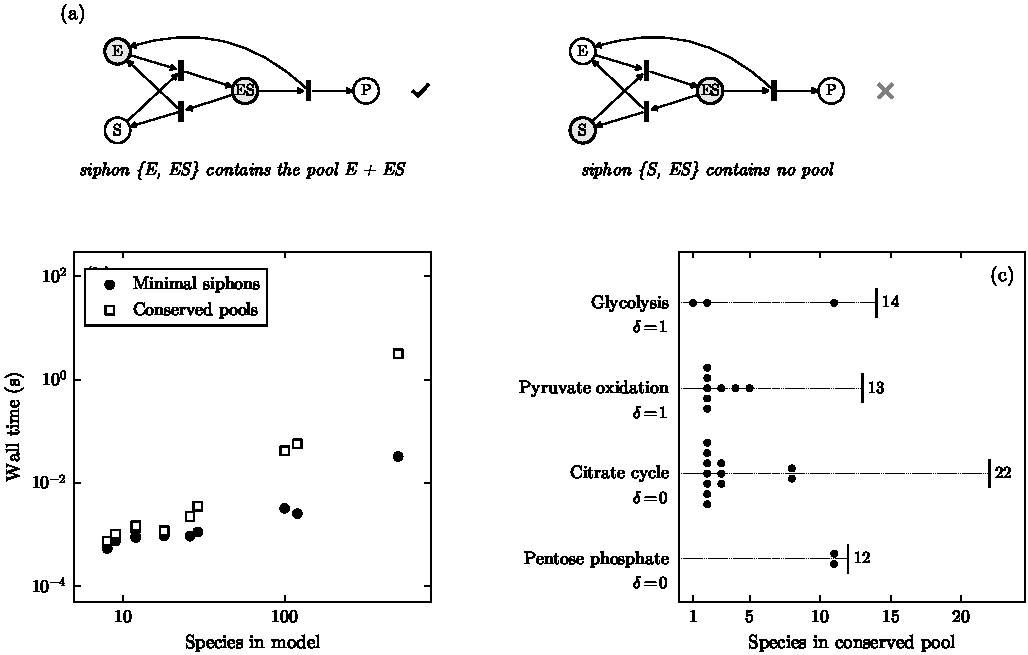
\includegraphics[width=\linewidth]{Figure/analysis_overview.pdf}
    \caption{Siphons and conserved pools, with C++ enumeration cost in \texttt{BioModels} and conserved pools in \texttt{KEGG} modules. \textbf{(a)}~The enzyme scheme of Figure~\ref{fig:synkit_architecture} as a Petri net (circles: species, bars: reactions, shaded: members of a minimal siphon). The siphon $\{E,ES\}$ contains the conserved pool $E+ES$, so it cannot become empty once marked (check). The siphon $\{S,ES\}$ contains no conserved pool and is not certified (cross). \textbf{(b)}~Wall time for completed minimal-siphon and exact conserved-pool enumeration in ten reaction-bearing models. All ten models complete both enumerations. \textbf{(c)}~Minimal non-negative conserved pools in four reduced modules. Each dot is one pool placed at its number of species, pools of equal size are stacked, and the dotted line spans the module species, ending at the module size.}
    \label{fig:evidence_overview}
\end{figure}

\subsection{Computational cost of exact structural enumeration}
\label{sec:results_scaling}

Figure~\ref{fig:scaling}b reports the repeated paired C++ experiment. Both algorithms return identical minimal siphons for every run. At 21 species, median exhaustive-search time is \ReviewExhaustiveMilliseconds~ms and median pruned-search time is \ReviewClosureMilliseconds~ms. The ratio of median times changes from \ReviewRatioSmall{} at 11 species to \ReviewRatioLarge{} at 21 species. The methods have comparable times at the smallest size, while exhaustive search becomes more expensive as the subset space grows. Quartiles describe repeat-to-repeat variation on these fixed networks, rather than variation across network topologies, and four sizes on one family do not establish asymptotic complexity.

The larger C++ sweep includes directed chains, reversible chains, and random sparse bimolecular networks (Supplementary Figure~\ref{supp:fig:performance_diagnostics}). All 60 requested configurations complete. On the 401-species reversible chain, minimal siphons take \ReviewReversibleSiphonSeconds~s, canonicalization \ReviewReversibleCanonicalSeconds~s, exact conserved pools \ReviewReversibleMoietySeconds~s, and standalone exact rank \ReviewReversibleRankSeconds~s (Figure~\ref{fig:scaling}c). The random-family networks with 49, 99, 197, and 395 species have 331, 272, 47, and 87 minimal siphons, respectively. At 395 species, siphon enumeration completes in \ReviewRandomSiphonSeconds~s and conserved-pool enumeration in \ReviewRandomMoietySeconds~s. These single-run measurements depend on topology, algorithm, and implementation. They establish neither a polynomial bound for enumeration nor a universal species-count ceiling.

\begin{figure}[!htbp]
\centering
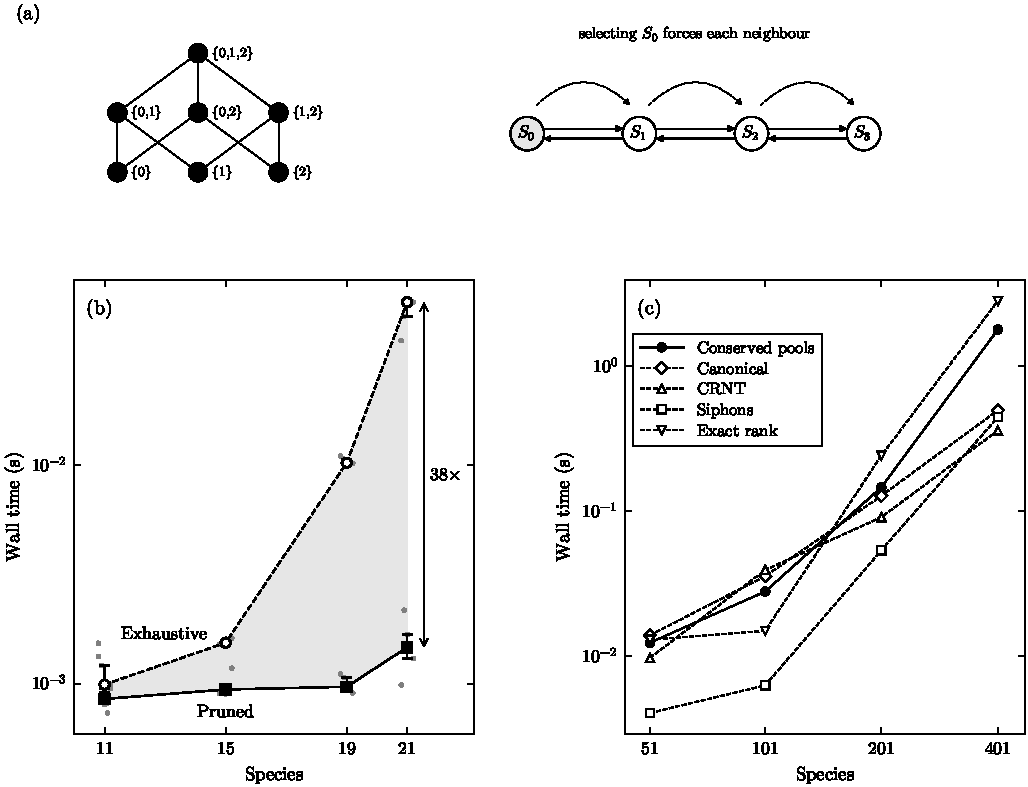
\includegraphics[width=\linewidth]{Figure/scaling.pdf}
\caption{C++ runtime comparison of siphon algorithms and structural analyses on reversible-chain networks. \textbf{(a)}~Exhaustive search tests every non-empty species subset. Implication pruning selects one species and propagates: every reaction producing a selected species must consume one, so in the reversible chain the selection of $S_0$ forces the whole chain, its only minimal siphon (dashed arrows). \textbf{(b)}~Exhaustive versus implication-pruned minimal-siphon enumeration across five repeats per size (points show individual runs, markers and error bars show medians and IQRs, and every pair returns identical siphon sets). Shading spans the gap between medians, and the bracket gives their ratio at 21 species. \textbf{(c)}~Single-run wall times for five analyses across larger reversible chains. Both panels include Python interface overhead, and lines connect successive sizes.}
\label{fig:scaling}
\end{figure}

\subsection{Structural \texttt{SBML} round-trip validation in \texttt{BioModels}}
\label{sec:results_biomodels}

A size-stratified manifest selects eleven \texttt{BioModels}~\cite{maliksheriff2020biomodels} entries comprising ten reaction-bearing models and one \texttt{SBML-qual} negative control. All ten pass the supported structural export/re-import checks, and their deficiency identities hold (Figure~\ref{fig:evidence_overview}b). Source identifiers, URLs, and input checksums accompany the results. The largest, \texttt{BIOMD0000000255}, contains 504 species and 827 directed reactions. Its C++ enumeration finds 75 minimal siphons and 17 minimal conserved pools in \ReviewBioModelSiphonSeconds~s and \ReviewBioModelMoietySeconds~s, respectively. All ten models complete both enumerations and their siphon-coverage checks; neither \texttt{BIOMD0000000255} nor the 100-species \texttt{BIOMD0000000019} (20 minimal siphons, 19 minimal conserved pools) satisfies the sufficient persistence condition. \texttt{BIOMD0000000562} is correctly diagnosed as reaction-free for Core structural analysis. The selected set tests interoperability over a range of sizes and does not estimate repository-wide support.

\subsection{Conservation and cofactor requirements in glycolysis}
\label{sec:results_kegg}

Four cached \texttt{KEGG}~\cite{kanehisa2025kegg} modules cover glycolysis (\texttt{M00001}), pyruvate oxidation (\texttt{M00307}), the citrate cycle (\texttt{M00009}), and the pentose phosphate pathway (\texttt{M00004}). Their conserved-pool supports appear in Figure~\ref{fig:evidence_overview}c. In the reduced citrate-cycle model, minimal non-negative conservation vectors recover nucleotide pairs, a quinone pair, a ferredoxin pair, coenzyme~A, and a lipoyl pool. Because these interpretations reflect the retained reaction equations and labels, they do not imply organism-specific physiological pool conservation.

The reduced glycolysis model has 14 species and 15 directed reactions ($n=16$, $\ell=4$, $s=11$, and $\delta=1$). Its largest minimal conservation support spans eleven carbohydrate intermediates, assigning weight two to hexoses and one to trioses (Figure~\ref{fig:glycolysis}). Glucose and oxidized ferredoxin form uncovered singleton siphons. Polyphosphate forms a covered singleton because the cached generic-polymer reaction retains it on both sides. This symbolic representation does not resolve polymer chain length or prove catalytic phosphate chemistry.

For one glucose token, the prescribed flux has a 15-step firing certificate ending in two pyruvate tokens, and search explores 30 states. The repeated lower-pathway firings are specified in the requested flux and are compatible with the two trioses produced by aldolase. Certificate replay verifies enabling at each step and conservation of the weighted carbohydrate pool. Requesting only the lower pathway from glucose fails because the required intermediates are absent.

\begin{figure}[!htbp]
    \centering
    % ---------------------------------------------------------------------------
% glycolysis.tex --- KEGG M00001 end to end: topology, exact structure, the
% returned firing certificate, and every recorded token marking.
%
% Source fragment: loaded directly by main.tex.
%
% Numerical macros are embedded in main.tex from analysis/glycolysis_analysis.json.
%
% Top panels show the reduced pathway and exact structural diagnostics.
% The full-width lower panel is generated from the complete recorded trajectory.
% ---------------------------------------------------------------------------
% Figure styles are supplied by the manuscript preamble.

\begingroup
% Use the full 16.40 cm manuscript width without stretching text or symbols.
\colorlet{scInk}{black}
\colorlet{scInkM}{black}
\renewcommand{\scBody}{\scArial\fontsize{7}{8.4}\selectfont\color{black}}
\renewcommand{\scSmall}{\scArial\fontsize{6.5}{7.8}\selectfont\color{black}}
% Carbon skeleton glyph: #1 carbon dots in a zigzag, #2 circled phosphates on
% the chain ends (as in Figures 5 and 6). Hexoses carry six dots and trioses
% three, so the weighted pool of panel b can be read off the drawing.
\newcommand{\gchain}[2]{\tikz[x=1cm,y=1cm,baseline=(gc1.base)]{%
  \foreach \i in {1,...,#1}{\pgfmathsetmacro\gy{mod(\i,2)*0.055}%
    \coordinate (gc\i) at ({(\i-1)*0.115},\gy);}%
  \draw[line width=0.5pt] (gc1) \foreach \i in {2,...,#1}{-- (gc\i)};%
  \foreach \i in {1,...,#1}{\fill (gc\i) circle (0.027);}%
  \ifnum#2>0 \draw[line width=0.35pt] (gc#1) -- ++(0,0.12)
    node[circle,draw,line width=0.35pt,fill=white,inner sep=0pt,
         minimum size=1.55mm,anchor=south,
         font=\scArial\fontsize{3.6}{3.6}\selectfont] {P};\fi
  \ifnum#2>1 \draw[line width=0.35pt] (gc1) -- ++(0,0.12)
    node[circle,draw,line width=0.35pt,fill=white,inner sep=0pt,
         minimum size=1.55mm,anchor=south,
         font=\scArial\fontsize{3.6}{3.6}\selectfont] {P};\fi
  \path (0,-0.05) (0,0.32);}}
\tikzset{
  % metabolite: carbon glyph over its abbreviation; the text names it
  gmet/.style={draw=none,fill=none,font=\scSmall,text=scInk,align=center,
               inner sep=1pt},
  gsmall/.style={rounded rectangle,fill=white,draw=black,line width=0.4pt,
                 font=\scSmall,text=scInk,minimum height=3.6mm,
                 inner xsep=2.0pt,inner ysep=1.0pt},
  gpath/.style={-{Stealth[round,length=1.9mm,width=1.5mm]},draw=figMuted,
                line width=0.8pt,shorten >=1.4pt,shorten <=1.4pt},
  gbypass/.style={-{Stealth[round,length=1.7mm,width=1.3mm]},draw=figMuted,
                  line width=0.6pt,dashed,shorten >=1.4pt,shorten <=1.4pt},
  % enzyme labels: 6 pt is the floor, and they knock out the edge behind them
  glabel/.style={font=\scSmall,text=scInkM,fill=white,inner sep=0.9pt},
}
% A siphon covered by a conservation law (teal check) or not (gray cross).
\newcommand{\gcov}{\textcolor{scAccent}{$\checkmark$}}
\newcommand{\gunc}{\textcolor{scInkM}{$\times$}}

\def\pw{6.415}
\def\qx{6.615}          % left edge of the right-hand column
\def\ry{-3.95}          % top edge of the bottom row

\begin{tikzpicture}[syn,x=1.258384cm]
\scCanvas{10.0}

% =========================================================================
% (a) module topology
%     upper chain -1.48 | lower chain -3.05 | note -3.95
% =========================================================================
\scHead{(0.22,-0.16)}{a}{}{}

\node[gmet] (glc)  at (0.55,-1.48) {\gchain{6}{0}\\Glc};
\node[gmet] (g6p)  at (1.92,-1.48) {\gchain{6}{1}\\G6P};
\node[gmet] (f6p)  at (3.29,-1.48) {\gchain{6}{1}\\F6P};
\node[gmet] (fbp)  at (4.56,-1.48) {\gchain{6}{2}\\FBP};
\node[gmet] (dhap) at (5.72,-1.05) {\gchain{3}{1}\\DHAP};
\node[gmet] (gap)  at (5.72,-2.08) {\gchain{3}{1}\\GAP};

% Labels ride above their edges: at 6 pt they do not fit between the nodes.
\draw[gpath] (glc) -- (g6p) node[glabel,midway,yshift=3.4mm] {HK $\times3$};
\draw[gpath] (g6p) -- (f6p) node[glabel,midway,yshift=3.4mm] {PGI};
\draw[gpath] (f6p) -- (fbp) node[glabel,midway,yshift=3.4mm] {PFK $\times2$};
\draw[gpath] (fbp) -- (dhap);
\node[glabel] at (5.03,-0.91) {ALD};
\draw[gpath] (fbp) -- (gap);
\draw[gpath] (dhap) to[out=-12,in=12,looseness=1.8] (gap);
\node[glabel] at (6.18,-1.64) {TPI};

\node[gmet] (bpg) at (5.20,-3.15) {\gchain{3}{2}\\BPG};
\node[gmet] (pg3) at (4.30,-3.15) {\gchain{3}{1}\\3PG};
\node[gmet] (pg2) at (3.40,-3.15) {\gchain{3}{1}\\2PG};
\node[gmet] (pep) at (2.50,-3.15) {\gchain{3}{1}\\PEP};
\node[gmet] (pyr) at (1.55,-3.15) {\gchain{3}{0}\\Pyr};

\draw[gpath] (gap) -- (bpg);
\node[glabel,anchor=west] at (5.62,-2.86) {GAPDH $\times2$};
\draw[gpath] (bpg) -- (pg3) node[glabel,midway,yshift=3.2mm] {PGK};
\draw[gpath] (pg3) -- (pg2) node[glabel,midway,yshift=3.2mm] {PGM};
\draw[gpath] (pg2) -- (pep) node[glabel,midway,yshift=3.2mm] {ENO};
\draw[gpath] (pep) -- (pyr) node[glabel,midway,yshift=3.2mm] {PK};

\node[catalyst,font=\scSmall,text=black] (poly) at (0.66,-2.42) {PolyP};
\draw[cat,dashed] (poly.north) to[out=80,in=-100] ($(glc)!0.50!(g6p)$);

\draw[gbypass] (gap.south) to[out=-80,in=18,looseness=1.1] (pg3.east);
\node[font=\scSmall,text=black,fill=white,inner sep=1pt] at (4.58,-3.78)
  {Fd$_{\rm ox}\!\to$Fd$_{\rm red}$ bypass};

% =========================================================================
% (b) exact structural fingerprint
%     stats -1.22 | moieties -2.28..-3.00 | law -3.20
%     | siphons -4.10 | verdict -4.40
% =========================================================================
\scHead{(\qx+0.22,-0.16)}{b}{}{}

\node[anchor=base west,font=\scBody,text=scInk] at (\qx+0.24,-1.12)
  {$n=\GlyComplexes$\qquad $\ell=\GlyLinkage$\qquad $s=\GlyRank$\qquad
   $\delta=\GlyDeficiency$};

% Conserved pools: one bar per minimal pool, length = species in the pool.
\foreach \i/\nm/\len/\val in {0/{carbohydrates}/3.15/\GlyBackboneSupport,
                              1/{Fd$_{\rm ox}$\,/\,Fd$_{\rm red}$}/0.573/2,
                              2/{PolyP}/0.286/1} {
  \pgfmathsetmacro{\byy}{-1.80-\i*0.36}
  \node[anchor=base east,font=\scSmall,text=scInkM] at (\qx+1.90,\byy) {\nm};
  \path[fill=npgBlue!70]
    (\qx+2.00,\byy-0.030) rectangle (\qx+2.00+\len,\byy+0.140);
  \node[anchor=base west,font=\scSmall,text=black]
    at (\qx+2.10+\len,\byy) {\val};
}

% Minimal siphons drawn as the species nodes of panel a, each with its verdict.
\node[anchor=base east,font=\scSmall,text=scInkM] at (\qx+1.90,-3.30) {siphons};
\node[gsmall] (s1) at (\qx+2.35,-3.25) {Glc};
\node[gsmall] (s2) at (\qx+3.45,-3.25) {PolyP};
\node[gsmall] (s3) at (\qx+4.65,-3.25) {Fd$_{\rm ox}$};
\node[anchor=west,inner sep=1pt] at (s1.east) {\gunc};
\node[anchor=west,inner sep=1pt] at (s2.east) {\gcov};
\node[anchor=west,inner sep=1pt] at (s3.east) {\gunc};

% (c) Full-width token map generated from the recorded certificate trajectory.
\node[anchor=north west,inner sep=0pt] at (0,\ry)
  {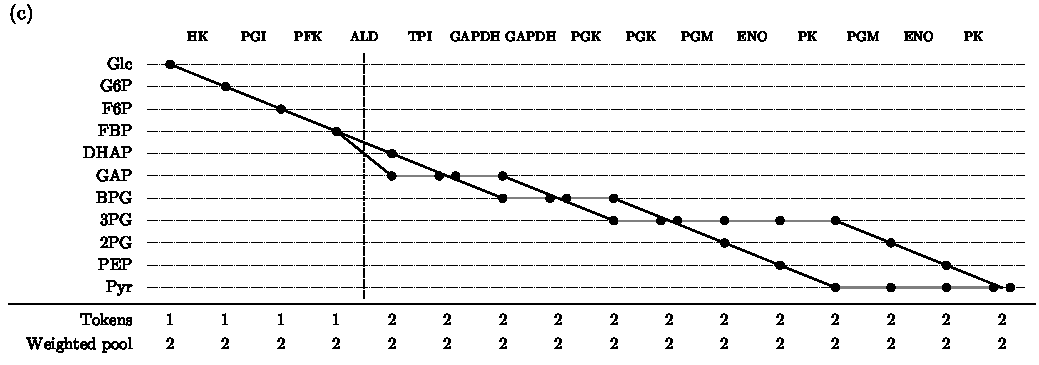
\includegraphics[width=16.4cm]{Figure/glycolysis_replay.pdf}};
\end{tikzpicture}
\endgroup

    \caption{Conserved pools and pathway realizability in reduced \texttt{KEGG} glycolysis (\texttt{M00001}). \textbf{(a)}~Bipartite network (14 species, 15 directed reactions, currency metabolites omitted) retaining shared polyphosphate and the ferredoxin bypass, where edge labels indicate parallel alternatives. Each metabolite is drawn as its carbon skeleton (dots: carbon atoms, circled P: phosphate), so hexoses carry six carbons and trioses three. \textbf{(b)}~Structural invariants, conserved pools (bar length: species per pool), and minimal siphons (check: covered by a conserved pool, cross: uncovered). The uncovered singleton siphons, glucose and oxidized ferredoxin, leave persistence uncertified. \textbf{(c)}~Token markings across the certified 15-step conversion of one glucose to two pyruvates (each dot is one token, lines link each consumed intermediate to its products, column labels name the enzyme fired, and the dashed line marks aldolase cleavage). Bottom rows trace total carbohydrate tokens and the conserved weighted pool ($2\times\text{hexoses} + 1\times\text{trioses} = 2$). Inactive polyphosphate and ferredoxin are omitted.}
    \label{fig:glycolysis}
\end{figure}

The controlled experiment isolates the information lost by cancellation (Figure~\ref{fig:representation}). Removing the common polyphosphate incidence from \texttt{R02189} preserves every species row, reaction column, and entry of $\mathbf S$. Consequently, its kernel and conservation space are unchanged. Yet the complex count changes from 16 to 14, linkage classes from four to three, and deficiency from one to zero. With one glucose and zero polyphosphate tokens, the retained reaction is blocked, whereas the cancelled reaction fires. Supplying one polyphosphate token enables the retained reaction. Two networks with the same net stoichiometric matrix can therefore differ in deficiency and in which reactions can fire.

A separate boundary control restores the currency metabolites, producing a 24-species model with the same 15 reactions. Under the same glucose-only inventory and requested flux, no reaction is enabled, because hexokinase lacks ATP, and exhaustive search returns \texttt{unrealizable}. The 15-step certificate therefore depends on currency removal. The reduced sequence establishes conversion of the carbohydrate intermediates, and evaluating cofactor sufficiency requires restoring the omitted species and specifying their initial amounts. Supplementary Section~\ref{supp:sec:si_case_glycolysis} gives a cofactor-coupled example with explicit ATP and ADP alternatives.

\begin{figure}[!htbp]
\centering
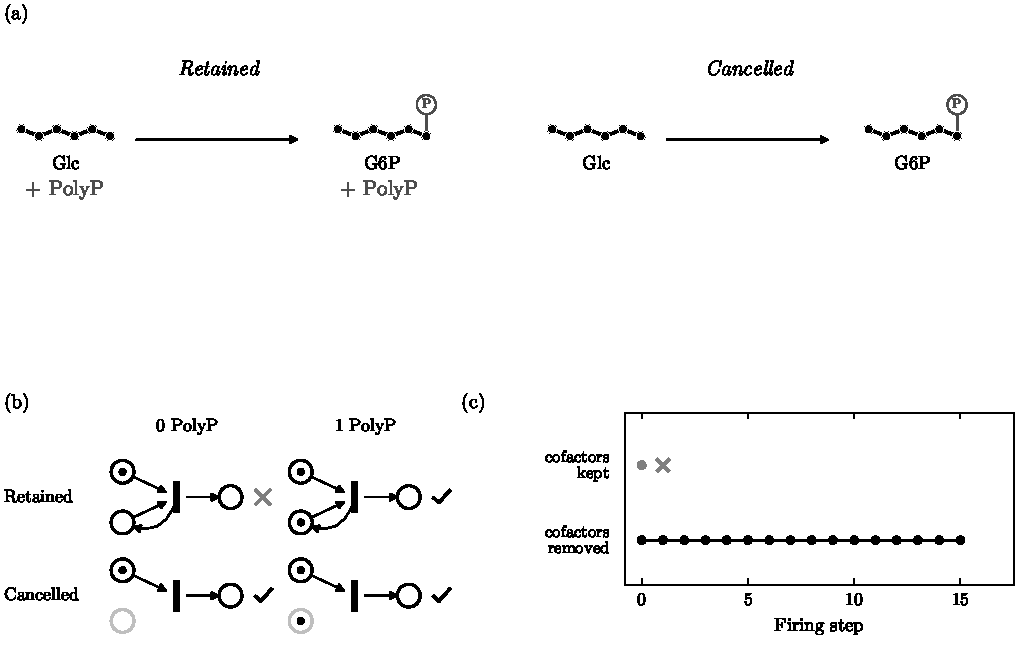
\includegraphics[width=\linewidth]{Figure/representation_sensitivity.pdf}
\caption{Sensitivity of structural invariants and pathway realizability to participant retention and currency omission. \textbf{(a)}~Cancelling shared polyphosphate (\texttt{PolyP}) in reaction \texttt{R02189} preserves net stoichiometry ($\mathbf S_{\mathrm{retained}} = \mathbf S_{\mathrm{cancelled}}$) but changes complex count ($n: 16 \to 14$), linkage classes ($\ell: 4 \to 3$), and deficiency ($\delta: 1 \to 0$). Glc indicates glucose, G6P indicates glucose 6-phosphate, filled circles represent carbon atoms, and P represents phosphate. \textbf{(b)}~\texttt{R02189} as a Petri net under zero or one \texttt{PolyP} token (upper input place: glucose, lower input place: \texttt{PolyP}, output place: G6P, dots: tokens). The retained reaction consumes and returns \texttt{PolyP}, so it fires only when a \texttt{PolyP} token is present (check: enabled, cross: blocked). \textbf{(c)}~Firing steps of the prescribed glycolytic flux from one glucose. With the currency metabolites (cofactors) kept in the model but not supplied (24 species), hexokinase lacks ATP, no reaction is enabled, and exhaustive search fails. With them removed (14 species), a certified 15-step sequence reaches two pyruvates.}\label{fig:representation}
\end{figure}

\subsection{Carbon conservation and precursor requirements in formose networks}
\label{sec:usecase_expand}

The formose reaction, in which formaldehyde condenses to a mixture of sugars~\cite{butlerov1861formose}, gives a rule-generated counterpart to the curated \texttt{KEGG} modules. Starting from formaldehyde and glycolaldehyde, four rules for aldol addition, retro-aldol cleavage, and reversible keto-enol tautomerization generate 37 species and 44 reactions after four iterations. Generation takes \ReviewFormoseGenerationSeconds~s in the C++ run and reaches species containing ten carbon atoms. The iteration count is a rule-expansion depth, not physical reaction time. The network has 54 complexes, 17 linkage classes, rank 36, and deficiency one.

Its one-dimensional left nullspace yields a positive primitive conservation vector. Comparing its coefficients with carbon counts from the molecular graphs gives exact agreement for all 37 species (Figure~\ref{fig:formose}). This is a consistency check between generated stoichiometry and molecular structures. Within this carbohydrate-only rule set, elemental counts can be proportional, but the result does not show that stoichiometry uniquely identifies elemental composition in general.

The hydrogen model of the expansion is a representation choice of the same kind as cancelling shared participants. With explicit hydrogen vertices, every hydrogen of a molecule is matched separately, and the hydrogen counts of product atoms are re-derived from default valences after each rule application. With hydrogens kept as per-atom counts, molecules are matched as heavy-atom graphs and product counts follow from the rule's hydrogen moves. Both models generate the same formose network after four, five, and six iterations. At six iterations (\HydrogenSpecies{} species and \HydrogenReactions{} reactions), expansion takes \HydrogenLewisSeconds~s with hydrogen counts and \HydrogenExplicitSeconds~s with hydrogen vertices. The models differ when a rule's hydrogen bookkeeping is incomplete or involves charged atoms with fixed hydrogen counts (Supplementary Table~\ref{supp:tab:hydrogen_models}). Re-deriving hydrogens turns a hydrogen-atom abstraction from ethane back into ethane, finds no reaction for a proton transfer from ammonium to acetate, and adds one hydrogen to each of the \HydrogenInsertionExplicit{} reactions of an incomplete alkene insertion rule. With hydrogen counts, all \HydrogenLewisReactions{} reactions of these three controls conserve atoms and charge, and the open valence left by the incomplete rule appears as a radical. Conservation analysis of a generated network therefore depends on hydrogen accounting during generation, before any stoichiometric matrix is formed.

\begin{figure}[!htbp]
    \centering
    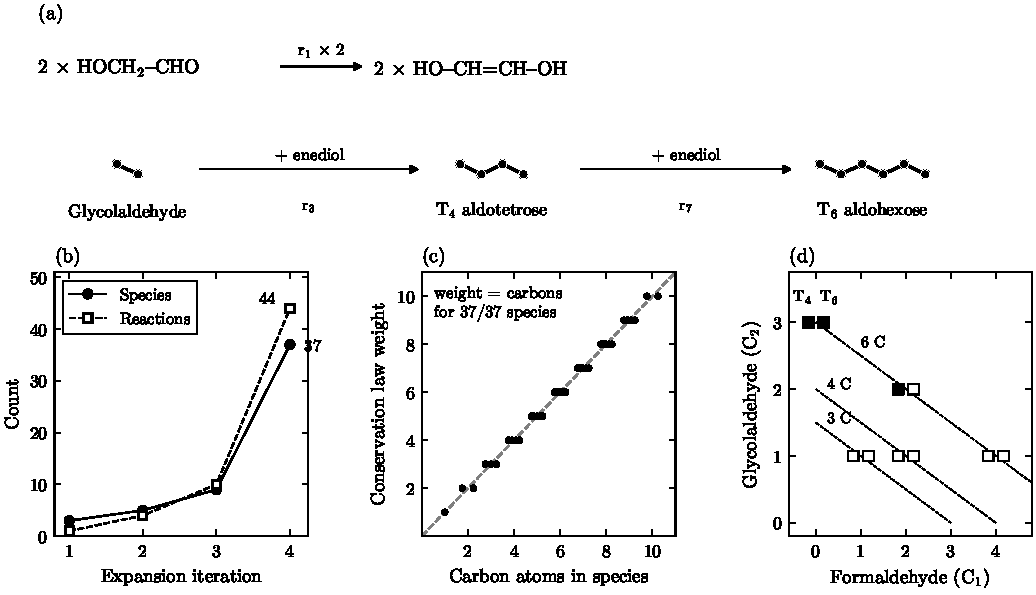
\includegraphics[width=\linewidth]{Figure/formose.pdf}
    \caption{Carbon conservation and precursor-dependent pathway realizability in the generated formose network. \textbf{(a)}~Target hexose route requiring three glycolaldehyde precursors via two enolizations ($r_1$) and two aldol additions ($r_3$, $r_7$), each addition consuming one enediol (filled circles: carbon atoms). \textbf{(b)}~Network growth across four rule-expansion iterations from formaldehyde and glycolaldehyde. \textbf{(c)}~Weights of the single conservation law against carbon atoms per species. They agree for all 37 species, which confirms that the generated reactions conserve carbon (points jittered horizontally, dashed line: $y=x$). \textbf{(d)}~Five initial inventories by formaldehyde and glycolaldehyde count, with dashed lines joining inventories of equal total carbon. The left and right squares of each inventory refer to the tetrose ($T_4$) and hexose ($T_6$) routes, filled when a certificate is verified and open when exhaustive search fails. Inventories with six carbon atoms differ in which routes they can supply.}
    \label{fig:formose}
\end{figure}

Qualitative search reaches representative tetrose and hexose targets from the two seed species, but realizability distinguishes inventories that share the same total carbon (Figure~\ref{fig:formose}d). With four formaldehyde and one glycolaldehyde molecule, neither selected route is realizable. With two of each precursor, the tetrose route is realizable but the hexose route is not. With three glycolaldehyde molecules, both are. Each of these inventories contains six carbon atoms. The selected routes therefore require suitable precursor multiplicities as well as a sufficient carbon budget. These results concern fixed reaction multisets in the generated network, and they do not establish unrestricted target unreachability or experimental synthetic feasibility. Supplementary Section~\ref{supp:sec:si_case_formose} gives the route definitions and initial pools.

\subsection{Comparison with existing reaction-network software}
\label{sec:comparison}

The methods in the CRN submodule are established and are also available in other packages. What the module adds is that one reaction record reaches all of them, so a conserved pool, a deficiency value, and a firing certificate refer to the same species set, the same treatment of shared participants, and the same boundary choices. Table~\ref{tab:software} places this scope alongside the packages closest to the analyses in this paper.

\begin{table}[!htbp]
\centering
\caption{Functional scope of biochemical reaction-network software (\yes{} documented, \pmark{} partial or indirect as detailed in footnotes, \no{} not documented). Feature presence is derived from package documentation and source code (for \texttt{MolFoundry}, its version~0.1 API documentation), and only \texttt{CRNT4SBML} was experimentally evaluated (Table~\ref{tab:reference}). The \synkit column describes its CRN submodule.}
\label{tab:software}
\footnotesize
\setlength{\tabcolsep}{4pt}
\renewcommand{\arraystretch}{1.12}
\begin{tabular*}{\linewidth}{@{\extracolsep{\fill}}l cccccccc@{}}
\toprule
 & \rot{\texttt{SynKit} (this work)}
 & \rot{\texttt{CRNT4SBML}~\cite{reyes2020crnt4sbml}}
 & \rot{\texttt{CoNtRol}~\cite{donnell2014control}}
 & \rot{\texttt{crnpy}~\cite{tonello2016crnpy}}
 & \rot{\texttt{COBRApy}~\cite{ebrahim2013cobrapy}}
 & \rot{\texttt{M\O D}~\cite{andersen2016mod}}
 & \rot{\texttt{MolFoundry}~\cite{friedrichs2026molfoundry}}
 & \rot{\texttt{Tellurium}~\cite{choi2018tellurium,welsh2023libroadrunner}} \\
\midrule
\multicolumn{9}{@{}l}{\emph{Network construction and exchange}}\\
\quad \texttt{KEGG} pathway ingestion                  & \yes & \no  & \no  & \no  & \no  & \no  & \no  & \no  \\
\quad \texttt{SBML} import                             & \pmark\textsuperscript{a} & \yes & \no & \yes & \yes & \no & \no & \yes \\
\quad \texttt{SBML} export                             & \pmark\textsuperscript{a} & \no  & \no  & \yes & \yes & \no  & \yes & \yes \\
\quad Rule-based generation from seeds        & \yes & \no  & \no  & \no  & \no  & \yes & \yes & \no  \\
\addlinespace[3pt]
\multicolumn{9}{@{}l}{\emph{Exact structural analysis}}\\
\quad Deficiency, linkage classes, weak reversibility & \yes & \yes & \yes & \yes & \no & \no & \no & \no \\
\quad Conservation laws (kernel basis)        & \yes & \yes & \no  & \yes & \no  & \no  & \no  & \yes \\
\quad Minimal P-semiflows (minimal support)   & \yes & \no  & \no  & \yes & \no  & \no  & \no  & \no  \\
\quad T-semiflows or elementary modes         & \yes & \no  & \no  & \yes & \no  & \no  & \no  & \no  \\
\quad Minimal siphons and traps               & \yes & \no  & \pmark\textsuperscript{b} & \no & \no & \no & \no & \no \\
\addlinespace[3pt]
\multicolumn{9}{@{}l}{\emph{Behavior and realizability}}\\
\quad Multistationarity or bistability search & \no  & \yes & \yes & \pmark\textsuperscript{c} & \no & \no & \no & \no \\
\quad Finite-inventory firing certificate     & \yes & \no  & \no  & \no  & \no  & \pmark\textsuperscript{d} & \yes\textsuperscript{f} & \no \\
\quad Constraint-based flux analysis          & \no  & \no  & \no  & \no  & \yes & \no  & \pmark\textsuperscript{f} & \no  \\
\quad Kinetic simulation                      & \no  & \pmark\textsuperscript{e} & \no & \no & \no & \no & \yes\textsuperscript{g} & \yes \\
\bottomrule
\end{tabular*}

\vspace{2pt}
\begin{minipage}{\linewidth}\footnotesize
\begin{tabular}{@{}r@{~}p{0.95\linewidth}@{}}
\textsuperscript{a} & \texttt{SBML} Level~3 Version~2 Core reaction structure and metadata only, as kinetic laws, events, rules, and package extensions are not handled. \\
\textsuperscript{b} & Siphons underlie \texttt{CoNtRol}'s persistence conditions, but minimal-siphon enumeration is not exposed as an output. \\
\textsuperscript{c} & \texttt{crnpy} supplies Gr{\"o}bner-basis, elementary-mode, and absolute-concentration-robustness machinery rather than a bistability search routine. \\
\textsuperscript{d} & \texttt{M\O D} provides an integer hyperflow model for pathway queries rather than a firing-sequence certificate over a finite marking. \\
\textsuperscript{e} & ODE simulation is provided in support of \texttt{CRNT4SBML}'s bistability analysis. \\
\textsuperscript{f} & \texttt{MolFoundry} solves integer hyperflow models over a derivation graph (Gurobi or SMT) and returns firing orders that realize a flow from its inflow marking. \\
\textsuperscript{g} & Rule-based stochastic simulation with on-demand network expansion. \\
\end{tabular}
\end{minipage}
\end{table}

Among the packages in Table~\ref{tab:software}, \texttt{crnpy} also provides exact semiflow analysis, and \texttt{MolFoundry}, which builds on the \texttt{M\O D} strategy framework, also generates networks from rules and returns firing orders for integer hyperflows. \synkitcrn combines rule-based construction, minimal siphons and traps, exact semiflows, and finite-inventory firing certificates (with exhaustive search for negative answers) in a single object. Bistability search, constraint-based flux analysis, and kinetic simulation require complementary tools such as \texttt{CRNT4SBML}, \texttt{CoNtRol}, \texttt{COBRApy}, and \texttt{Tellurium}.

The external evaluation tests agreement with \texttt{CRNT4SBML} on shared CRNT outputs rather than comparing usability, end-to-end runtime, or non-overlapping features across packages.

\subsection{Model assumptions and computational limitations}
\label{sec:limitations}

The conclusions depend on the reaction list, cofactor treatment, reversibility, and boundary species. The glycolysis controls quantify two consequences of changing these assumptions. Minimal-semiflow and siphon enumeration can have combinatorial output and runtime growth. Timeouts and incomplete search must remain visible. None of the analyses predicts kinetic rates, thermodynamic driving forces, or in vivo activity. Future work should prioritize broader input validation and scalable exact enumeration with explicit resource reporting.

\section{Conclusions}
\label{sec:discussion}

The CRN submodule of \synkit applies exact conservation analysis, deficiency theory, and firing certificates to curated and rule-generated reactions alike. Reference checks and an external \texttt{SBML} comparison support its structural computations, while metabolic and formose examples show how to interpret the outputs. The controlled glycolysis experiment demonstrates why preserving reactant and product incidence matters even when net stoichiometry is unchanged. Together, the analyses identify conserved metabolite pools and test whether specified substrate amounts support a proposed reaction sequence. Their interpretation remains conditional on the biochemical species and reactions included in the model.


\section*{Availability and requirements}
\begin{itemize}[leftmargin=*,label={},itemsep=0pt]
\item \textbf{Project name:} \synkit (CRN submodule)
\item \textbf{Project home page:} \href{https://github.com/TieuLongPhan/SynKit}{github.com/TieuLongPhan/SynKit}
\item \textbf{Software version:} \synkit~1.6.5~\cite{synkit165release}
\item \textbf{Operating system(s):} Platform independent. The test suite runs on Linux, macOS, and Windows, and the reported analyses were run on Linux
\item \textbf{Programming language:} Python, C++17 (analysis library), and C++20 (rule expander)
\item \textbf{Other requirements:} Python~3.10 or higher, \texttt{NetworkX}~3.3 or higher, \texttt{NumPy}, \texttt{SciPy}, \texttt{RDKit}, a C++17 compiler, and Boost headers. Native rule expansion additionally requires CMake, a C++20 compiler, and an RDKit C++ installation
\item \textbf{License:} MIT
\item \textbf{Any restrictions to use by non-academics:} None
\end{itemize}

\section*{List of abbreviations}
ACR: absolute concentration robustness.
CRN: chemical reaction network.
CRNT: chemical reaction network theory.
DPO: double pushout.
EMP: Embden-Meyerhof-Parnas.
\texttt{KEGG}: Kyoto Encyclopedia of Genes and Genomes.
\texttt{SBML}: Systems Biology Markup Language.
\texttt{SMARTS}: SMILES arbitrary target specification.
TCA: tricarboxylic acid.
WR: weakly reversible.

\section*{Declarations}

\subsection*{Ethics approval and consent to participate}
Not applicable.

\subsection*{Consent for publication}
Not applicable.


\subsection*{Availability of data and materials}
The CRN submodule is distributed with \synkit.
Source code is available on GitHub at \href{https://github.com/TieuLongPhan/SynKit}{github.com/TieuLongPhan/SynKit}, including the v1.6.5 release~\cite{synkit165release}. Installation is available via PyPI at \href{https://pypi.org/project/synkit/}{pypi.org/project/synkit/}, and documentation is hosted at \href{https://tieulongphan.github.io/SynKit/}{tieulongphan.github.io/SynKit/}. The earlier v1.6.2 release is archived on Zenodo~\cite{synkit162archive}.
\synkit is released under the MIT License.
The \synkit{} numerical results and timings reported here were regenerated on 6 November 2026 using the version~1.6.5 source checkout (commit \texttt{5951b401b161}) and the script \texttt{analysis/scripts/regenerate\_evidence.py}, which runs every study, the external comparison, and the structural cross-checks, and installs the reports read by the manuscript. The accompanying JSON evidence records the analysis environment, the hashes of all CRN source files, native build identifiers for the analysis library and the rule expander, and input data. The comparison with \texttt{CRNT4SBML} reuses its recorded outputs after verifying that all twelve exported \texttt{SBML} inputs have identical checksums and that the recomputed \synkit~1.6.5 quantities agree. The legacy comparator interpreter was not rerun.
The \texttt{KEGG} module records underlying Figure~\ref{fig:evidence_overview}c are derived from \texttt{KEGG}~\cite{kanehisa2025kegg} and cached for reproducibility, so they are not covered by \synkit's MIT license and remain subject to \texttt{KEGG}'s terms. The \texttt{BioModels} inputs are identified and checksum-recorded in the evidence, while \texttt{BioModels} distributes its dataset under the CC0 1.0 Public Domain Dedication.

\subsection*{Use of generative AI}
Claude Opus 5.5 (Anthropic) was used for language editing, journal formatting, plotting-code revisions, the native rule-expansion program and its hydrogen-count model, and the evidence regeneration script. Codex (OpenAI) assisted with the C++ implementation, execution of the reproducible analysis scripts, and regeneration of numerical results and figures. Numerical results were computed by analysis code from recorded inputs. The authors are responsible for reviewing the code, results, and manuscript.

\subsection*{Competing interests}
The authors declare that they have no competing interests.

\subsection*{Funding}
This project has received funding from the European Union's Horizon Europe
Doctoral Network programme under the Marie-Sk{\l}odowska-Curie grant agreement
No~101072930 (TACsy, Training Alliance for Computational systems chemistry).
Views and opinions expressed are however those of the author(s) only and do not necessarily reflect those of the European Union. Neither the European Union nor the granting authority can be held responsible for them.

\subsection*{Authors' contributions}
Author contributions are reported using the CRediT taxonomy. \textbf{T.-A.P.}: Software, Validation, Writing (original draft), Writing (review and editing). \textbf{T.-L.P.}: Conceptualization, Methodology, Software, Validation, Writing (original draft), Writing (review and editing). Both authors read and approved the final manuscript.

\subsection*{Acknowledgements}
Not applicable.

% Bibliography
\bibliography{refs}

\end{document}
